\documentclass[11pt,letterpaper]{article}

% Packages
\usepackage[margin=0.75in]{geometry}
\usepackage{graphicx}
\usepackage{xcolor}
\usepackage{tikz}

% Colors - Clean, professional
\definecolor{primaryblue}{RGB}{0, 102, 204}
\definecolor{accentgreen}{RGB}{46, 184, 92}
\definecolor{warningred}{RGB}{220, 53, 69}
\definecolor{lightgray}{RGB}{248, 249, 250}
\definecolor{textgray}{RGB}{73, 80, 87}

% Setup
\pagestyle{empty}
\setlength{\parindent}{0pt}
\setlength{\parskip}{8pt}

% Custom commands
\newcommand{\checkbox}{\tikz[baseline=-0.5ex]{\draw[line width=0.8pt] (0,0) rectangle (0.32,0.32);}\hspace{0.2em}}
\newcommand{\sectionbar}[1]{%
    \vspace{0.15cm}
    \noindent\colorbox{primaryblue}{%
        \parbox{\dimexpr\textwidth-2\fboxsep\relax}{%
            \textcolor{white}{\large\bfseries\sffamily #1}%
        }%
    }
    \vspace{0.2cm}
}

\begin{document}

% Header
\begin{center}
    {\LARGE\bfseries\sffamily\color{primaryblue} EVENITY (ROMOSOZUMAB)}\\[0.1cm]
    {\large\sffamily Prior Authorization Checklist}\\[0.15cm]
    \rule{0.5\textwidth}{0.5pt}\\[0.1cm]
    {\small Prepared for Lamar Health | Edward Zhong | edward.zhong@example.com}
\end{center}

% Quick Reference
\noindent
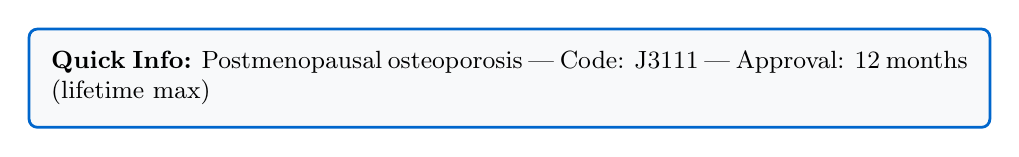
\begin{tikzpicture}
    \node[draw=primaryblue, line width=1pt, fill=lightgray, rounded corners=3pt, inner sep=8pt] {
        \begin{minipage}{0.96\textwidth}
            \small
            \textbf{Quick Info:} Postmenopausal osteoporosis | Code: J3111 | Approval: 12 months (lifetime max)
        \end{minipage}
    };
\end{tikzpicture}

\sectionbar{APPROVAL CRITERIA (Complete each section in order)}

\textbf{\large Section 1:} \textcolor{primaryblue}{\textbf{Patient Demographics \& Diagnosis}}

\checkbox\ Postmenopausal woman with osteoporosis?

\checkbox\ T-score $\leq$ -2.5 \textbf{OR} documented high fracture risk?

\hspace{2em}\textcolor{warningred}{$\triangleright$ If either is NO $\rightarrow$ \textbf{DENY}}

\textbf{\large Section 2:} \textcolor{primaryblue}{\textbf{Prior Treatment (need ONE pathway)}}

\textbf{Standard Pathway:}
\begin{itemize}
    \item[\checkbox] Failed 2 oral bisphosphonates (alendronate, ibandronate) \textbf{OR}
    \item[\checkbox] Failed 1 oral bisphosphonate + Reclast (IV zoledronic acid) \textbf{OR}
    \item[\checkbox] Failed 1 oral bisphosphonate + Prolia (denosumab)
\end{itemize}

\textbf{Continued Fracture Pathway:}
\begin{itemize}
    \item[\checkbox] Severe osteoporosis with continued fracture after 1 year continuous bisphosphonates
\end{itemize}

\textbf{Fast-Track Pathway:}
\begin{itemize}
    \item[\checkbox] Severe osteoporosis (T-score $\leq$ -3 \textbf{OR} multiple vertebral fractures)
    \item[\checkbox] Evidence supporting maximized bone density with Evenity before bisphosphonates/Prolia
\end{itemize}

\hspace{2em}\textcolor{warningred}{$\triangleright$ If NO pathways met $\rightarrow$ \textbf{DENY}}

\textbf{\large Section 3:} \textcolor{primaryblue}{\textbf{Exclusion Check (ALL must be clear)}}

\checkbox\ Patient is \textbf{NOT} on combination bone density therapy

\checkbox\ Patient does \textbf{NOT} have osteopenia (must be osteoporosis)

\checkbox\ Patient has \textbf{NOT} been treated with Forteo or Tymlos

\hspace{2em}\textcolor{warningred}{$\triangleright$ If ANY flags $\rightarrow$ \textbf{DENY}}

\noindent
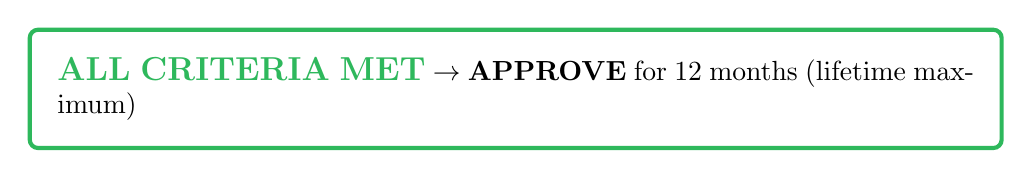
\begin{tikzpicture}
    \node[draw=accentgreen, line width=1.5pt, fill=white, rounded corners=3pt, inner sep=10pt] {
        \begin{minipage}{0.96\textwidth}
            \textcolor{accentgreen}{\large\bfseries ALL CRITERIA MET} $\rightarrow$ \textbf{APPROVE} for 12 months (lifetime maximum)
        \end{minipage}
    };
\end{tikzpicture}

\newpage

\sectionbar{HOW I USED AI (Claude)}

\textbf{The Process}

I asked Claude: \textit{"Extract all approval criteria from this Evenity policy and structure them as a decision tree."} It gave me comprehensive, accurate extraction (I verified against source), but the nested tree was optimized for completeness, not usability. A pharmacy tech would need 2-3 minutes to navigate it.

This taught me something: AI gives you what you ask for, not what users need.

\textbf{The Hard Part}

The trickiest challenge was figuring out how criteria 1.3, 1.4, and 1.5 relate. Are they cumulative (need all three) or alternative pathways (need just one)?

Reading the policy, I formed a hypothesis: the structure "1.3 OR 1.4 OR 1.5" and phrase "any of the following" suggested alternatives - different patient populations qualify different ways.

I needed to verify before building around it. I asked Claude: \textit{"Criteria 1.3, 1.4, and 1.5 - are these cumulative or alternative? Do patients need all three or just one?"}

Claude confirmed: separate pathways (OR logic). Getting this wrong means either denying eligible patients or approving ineligible ones - that's the stakes in healthcare.

\textbf{The Design}

With the logic clear, I restructured it: 3 sections with fail-fast logic (stop as soon as something doesn't qualify). Three distinct pathway boxes in Section 2 making it immediately clear which route applies. Structure mirrors both how the code would work and how someone would actually use it.

Bottom line: AI handles grunt work and validates reasoning. You own the product decisions - understanding users, knowing what's useful vs. just correct. That's the collaboration.

\sectionbar{ABOUT ME}

I'm Edward, recent UCSB CS grad. I've shipped production systems (invoice automation, AI tools), but what I'm actually good at is the translation work - taking messy, complex domains and building tools that non-technical people want to use.

That's the FDE role. Be with users. Understand what's broken. Build something that fixes it. Ship it. Get feedback. Make it better. I want to do that for healthcare - not because I know healthcare (I don't), but because I know how to learn domains from users and turn problems into working software.

Lamar is fixing genuinely broken infrastructure. Prior auth paperwork delays patients getting their meds. That's real impact. I want to help build the tools that actually work.

\begin{center}
\rule{0.7\textwidth}{0.5pt}\\[0.15cm]
{\small\textcolor{textgray}{Looking forward to the conversation | Edward Zhong}}
\end{center}

\end{document}